\documentclass[oneside,12pt,french,table]{book}
\usepackage[french]{babel}

%
% === S4S Theme ===
%

% Page format
\usepackage[margin=1in]{geometry}

% Custom fonts. This package is only available with XeLaTex (pdflatex is a mess to deal with)
\usepackage{fontspec}
\setmainfont{GeneralSans}[
    Path = assets/fonts/,
    Extension = .otf,
    UprightFont = *-Regular,
    ItalicFont = *-Italic,
    BoldFont = *-Bold,
    BoldItalicFont = *-BoldItalic
]

% Colors
\usepackage{xcolor}
\definecolor{S4S-light}{HTML}{50527F}
\definecolor{S4S-accent}{HTML}{2C2C5C}

% Title customization
\usepackage{titling}

% Fancy chapters
\usepackage[Bjornstrup]{fncychap}
\ChTitleVar{\Large\flushright\bfseries}

% Theorem styling and environments
\usepackage{amsthm}
\theoremstyle{definition}
\newtheorem{definition}{Définition}[chapter]
\theoremstyle{plain}
\newtheorem{theorem}[definition]{Théorème}
\newtheorem{corollaire}[definition]{Corollaire}
\theoremstyle{remark}
\newtheorem{remark}[definition]{Remarque}

% Boxed theorems
\usepackage{tcolorbox}
\newenvironment{greybox}{%
    \begin{tcolorbox}[boxrule=0pt, frame empty]
}{\end{tcolorbox}}

\newenvironment{boxdef}{%
    \begin{greybox}
    \begin{definition}
}{
    \end{definition}
    \end{greybox}
}

\newenvironment{boxthm}{%
    \begin{greybox}
    \begin{theorem}
}{
    \end{theorem}
    \end{greybox}
}

\newenvironment{boxcorollary}{
    \begin{greybox}
    \begin{corollaire}
}{
    \end{corollaire}
    \end{greybox}
}

% Paragraph spacing
\usepackage{parskip}

%
% === Math packages ===
%

% Default mathematical packages
\usepackage{amsmath}
\usepackage{amsfonts}

% Custom commands
\newcommand{\eqdef}{\stackrel{\textrm{déf.}}{=}}

% Graphics
\usepackage{tikz}
\usetikzlibrary{decorations.pathreplacing,calligraphy} % curly braces
\usepackage{float} % for float positioning, in particular the H modifier
\usepackage{subcaption} % for subfigures and subcaptions
\usepackage{pgfplots}
\pgfplotsset{compat=newest}
\pgfplotsset{%
  every tick label/.append style = {font=\tiny},
  every axis label/.append style = {font=\scriptsize}
}
\usetikzlibrary{plotmarks}

\usepackage{tkz-tab} % sign tables

% Clickable links
% (hyperref should stay the last import in most cases)
\usepackage[colorlinks,allcolors=S4S-light,linktocpage]{hyperref}

\title{Cours d'Analyse}
\renewcommand{\maketitlehookb}{
    \begin{center}
    
\includegraphics[scale=0.5]{assets/imgs/logo-round.png}
    \end{center}
}

\author{Students 4 Students}
\date{Septembre 2023}

\begin{document}

\maketitle

\tableofcontents

\setcounter{chapter}{-1} % to start at Chapter 0
\chapter{Introduction}
Salut ! Ce document résume le contenu du cours d'Analyse de Students 4 Students, édition 2022. Il a été écrit dans le but de t'aider à te souvenir du cours, que ce soit pour les séries d'exercices ou pour un usage futur. Ainsi, les explications qui y sont faites sont minutieusement développées, à l'instar de ce qui a été fait durant les 4 heures de cours. Tu y trouveras aussi des ressources supplémentaires pour pouvoir perfectionner ta compréhension du cours.

\smallskip
En te souhaitant une bonne lecture,
\smallskip

\hfill L'équipe Analyse S4S.
\chapter{Rappels et fondamentaux}
% - Rappels sur les ensembles, introduction des ensembles N et R et notation $x \in A$
% - Rappels sur la valeur absolue, distance et inégalité triangulaire

Dans cette section, on introduit quelques notions fondamentales nous seront utiles pour les chapitres suivants.

\section{Ensembles}

\begin{boxdef}[Ensemble]
Un \emph{ensemble} $A$ est une collection non ordonnée d'éléments uniques. On note
\begin{equation}
A = \{x_1, x_2, \ldots, x_n\}
\end{equation}
pour l'ensemble contenant exactement les éléments $x_1$ jusqu'à $x_n$.
\end{boxdef}
Pour le cours, nous n'aurons pas besoin de définir plus rigoureusement ce qu'est un ensemble que la définition ci-dessus. Notez cependant qu'une majeure partie de la théorie mathématique se base sur cette notion fondamentale, et que vous la rencontrerez de manière plus formelle assez rapidement dans votre cursus.

On note $x \in A$ pour l'appartenance de $x$ à l'ensemble $A$. Naturellement, il nous suffit de barrer le symbole, i.e. $x \not\in A$, pour signifier que $x$ n'est pas un élément de $A$.

On définit la notion de \emph{sous-ensemble} de la même manière qu'on définirait une sous-collection~:
\begin{boxdef}[Sous-ensemble]
Un \emph{sous-ensemble} $B$ d'un ensemble $A$ est un ensemble tel que tous les éléments de $B$ sont des éléments de $A$. Symboliquement~:
\begin{equation}
\forall x \in B, x \in A
\end{equation}
On note $B \subseteq A$ pour signifier que B est un sous-ensemble de A.
\end{boxdef}

\subsection{Ensembles usuels}
Certains ensembles seront utilisés fréquemment par la suite, et ils sont tellement utiles en mathématiques qu'ils méritent une notation spéciale à eux seuls.

\begin{greybox}
\textbf{Ensembles usuels.}
\begin{enumerate}
    \item \emph{L'ensemble vide}, i.e. qui ne contient aucun élément, est noté $\emptyset$.
    \item L'ensemble des \emph{entiers non-négatifs} est l'ensemble des nombres positifs auquel on ajoute le nombre $0$\footnote{En mathématiques, on distingue la notion de \emph{nombre positif}, qui ne contient pas $0$, de celle de nombre \emph{non-négatif}, qui elle accepte $0$. Par convention, 0 n'est donc ni négatif, ni positif.}. On le note
    \begin{equation}
    \mathbb{N} = \{0, 1, 2, \ldots\}
    \end{equation}
    
    \item L'ensemble des \emph{entiers relatifs} est l'ensemble des nombres positifs, négatifs ou nuls. On le note
    \begin{equation}
    \mathbb{Z} = \{\ldots, -2, -1, 0, 1, 2, \ldots\}
    \end{equation}
    
    \item L'ensemble des \emph{nombres rationnels} est l'ensemble des fractions, de la forme $\frac{p}{q}$, où $p, q$ sont des entiers relatifs, $q \neq 0$. On le note $\mathbb{Q}$.
    
    \item L'ensemble des \emph{nombres réels} contient l'ensemble des nombres rationnels, ainsi que tous les nombres \emph{irrationels} (c'est-à-dire ne pouvant pas s'écrire comme une fraction rationnelle), tels que $\pi$, $e$, $\sqrt{2}$, etc. On le note $\mathbb{R}$.
    
    \item L'ensemble des \emph{nombres complexes} est l'ensemble des nombres de la forme $a + ib$, où $a, b$ sont des nombres réels, et $i$ est défini par $i = \sqrt{-1}$. On le note $\mathbb{C}$.
\end{enumerate}
\end{greybox}

Notons que rien ne nous a empêché de définir un ensemble infini comme une collection infinie, et qu'on a abusé des points de suspension pour pouvoir définir ces ensembles de manière plus aisée.

\subsection{Intervalles réels}
Les intervalles réels sont des sous-ensembles spéciaux de $\mathbb{R}$, qui sont définies par deux bornes. Ils contiennent tous les nombres entre ces deux bornes, ainsi que potentiellement les bornes elles-mêmes. On note ainsi
\begin{greybox}
\textbf{Notations des intervalles}.
Soit $a < b$ deux nombres réels.
\begin{enumerate}
    \item $[a, b]$ est l'ensemble des nombres réels $x$ tels que $a \leq x \leq b$
    \item $[a, b[$ est l'ensemble des nombres réels $x$ tels que $a \leq x < b$
    \item $]a, b]$ est l'ensemble des nombres réels $x$ tels que $a < x \leq b$
    \item $]a, b[$ est l'ensemble des nombres réels $x$ tels que $a < x < b$
\end{enumerate}
Si l'une des deux bornes est $\pm \infty$, on note alors
\begin{enumerate}
    \item $]\!-\!\infty, b]$ pour l'ensemble des nombres réels $x$ tels que $x \leq b$
    \item $]\!-\!\infty, b[$ pour l'ensemble des nombres réels $x$ tels que $x < b$
    \item $[a, \infty[$ pour l'ensemble des nombres réels $x$ tels que $a \leq x$
    \item $]a, \infty[$ pour l'ensemble des nombres réels $x$ tels que $a < x$
\end{enumerate}
\end{greybox}
Certains intervalles réels ont des notations particulières~:
\begin{greybox}
\begin{enumerate}
    \item $\mathbb{R}^+ = [0, \infty[$ est l'ensemble des nombre réels non-négatifs.
    \item $\mathbb{R}^- = \,]\!-\!\infty, 0]$ est l'ensemble des nombres réels non-positifs.
    \item $\mathbb{R}^* = \,]\!-\!\infty, 0[ \cup ]0, \infty[$  est l'ensemble des nombres réels non-nuls.
\end{enumerate}
\end{greybox}
et similairement $\mathbb{R}^{*+} = \,]0, \infty[$ pour l'ensemble des nombres réels positifs, $\mathbb{R}^{*-} = \,]\!-\!\infty, 0[$ pour l'ensemble des nombres réels négatifs.

\section{Valeur absolue, inégalité triangulaire}
Pour n'importe quel nombre réel $x \in \mathbb{R}$, on définit sa \emph{valeur absolue} comme la valeur non-négative qui est obtenue en enlevant le signe $+$ ou $-$ de son écriture décimale~:
\begin{boxdef}[Valeur absolue]
La \emph{valeur absolue} de $x \in \mathbb{R}$ est la valeur non-négative notée $|x|$ et définie par~:
\begin{equation}
|x| = \begin{cases}
x & \textrm{si } x \geq 0 \\
-x & \textrm{si } x < 0
\end{cases}
\end{equation}
\end{boxdef}
Vue sous un autre angle, la valeur absolue d'un nombre est sa \emph{distance} à 0, si on place le point sur la droite réelle~:
\begin{figure}[H]
    \centering
    \begin{tikzpicture}
    \draw[->] (-2, 0) to (5, 0) node[right] {$\mathbb{R}$};
    \node[circle,fill,inner sep=1pt,label={$0$},draw] (a) at (0,0){};
    \node[circle,fill,inner sep=1pt,label={$x$}, draw] (b) at (3, 0){};
    \draw[decorate, decoration = {calligraphic brace,raise=2pt,amplitude=3pt}] (b.center) -- (a.center) node[pos=0.5,below]{$|x|$};
    \end{tikzpicture}
    \caption{Droite réelle et valeur absolue}
    \label{fig:abs_real_axis}
\end{figure}
Cette notion de distance à 0 est importante, car elle permet de définir la distance \emph{entre deux nombres réels} quelconques $x, y \in \mathbb{R}$ par $d(x, y) = |x - y|$. Puisque $|x-y|$ est la distance de $x - y$ à 0, si $|x-y| = d$ alors $x - y = \pm d$, i.e. $x = y \pm d$, et ainsi $d$ est la distance entre $x$ et $y$.

Une inégalité fondamentale est \emph{l'inégalité triangulaire}~:
\begin{boxdef}[Inégalité triangulaire]
Pour tout $x, y \in \mathbb{R}$~:
\begin{equation}
|x + y| \leq |x| + |y|
\end{equation}
\end{boxdef}
Autrement dit, si l'on additionne deux nombres réels $x, y$, alors la distance à 0 de leur somme ne peut être plus grande que la somme des distances à 0 de $x$ et $y$, prises séparément. On peut se convaincre de la validité de l'inégalité triangulaire en utilisant un graphique similaire à la Figure \ref{fig:abs_real_axis} (essayez par vous-même pour vous convaincre).
\chapter{Suites numériques}

\label{chap:suite}
\section{Introduction~: Une histoire de lapins}
On considère des couples (inséparables) de lapins. Cette population évolue au fil des mois selon les règles suivantes~:
\begin{enumerate}
    \item Au début du premier mois, il y a un unique couple de lapins nouveau-nés.
    \item Au début de chaque nouveau mois, tout couple ayant vécu au moins 2 mois entiers donne naissance à un nouveau couple de bébés lapins.
    \item Les lapins sont immortels.
\end{enumerate}
L'image \ref{fig:rabbits} montre l'évolution des couples de lapins au fil des premiers mois.
\begin{figure}[H]
\centering 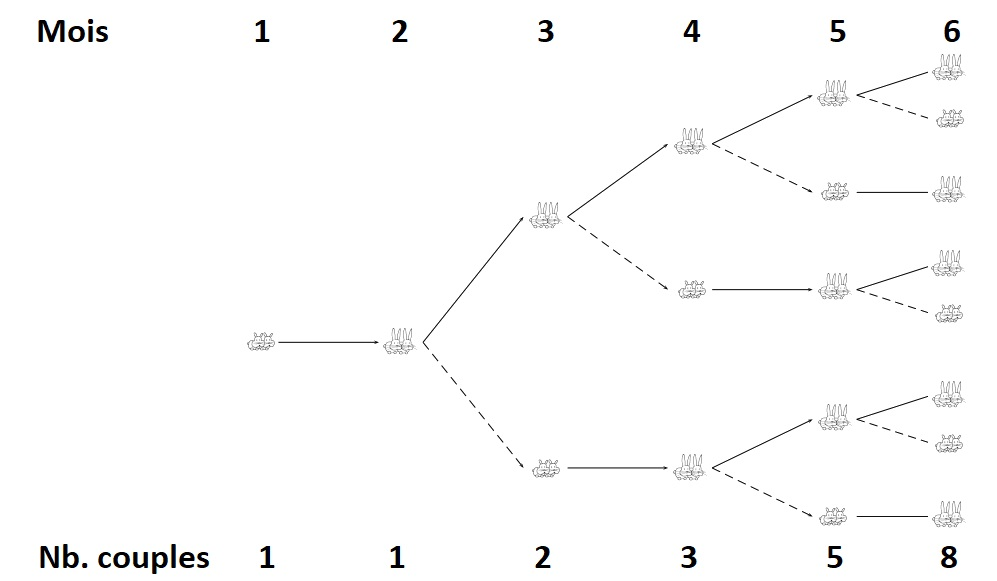
\includegraphics[width = 0.85\textwidth]{./assets/imgs/rabbit_tree.jpg}
\caption{Les couples de lapins au fil des 6 premiers mois}
\label{fig:rabbits}
\end{figure}

\begin{greybox}
\textbf{Question 1.} Combien de couples de lapins y a-t-il au mois numéro $n$ ? Ici, $n$ peut être n'importe quel nombre entier positif~: $n = 1, 2, 36, 1002,$ etc\textellipsis

On souhaite avoir une définition générale pour décrire le nombre de couples au $n$-ième mois, que l'on va dénoter $x_n$. 
\end{greybox}

\begin{boxdef}[Suite]
Une telle séquence de nombres réels $x_1, x_2, x_3, ...$, indexée par les entiers positifs de $\mathbb N$, est appelée \emph{suite}. On la note $(x_n)_{n \in \mathbb{N}^*}$, $(x_n)_{n \geq 1}$, ou simplement $(x_n)$, et on note $x_n$ le $n$-ième élément de la suite.
\label{def:suite}
\end{boxdef}

\begin{greybox}
\textbf{Question 2.} Quel est le comportement de $x_n$ quand $n$ devient grand ? Est-ce que $x_n$ devient très grand lui aussi ? Est-ce que $x_n$ oscille entre certaines valeurs ? Est-ce que $x_n$ se stabilise vers une valeur précise ? Ce sont quelques exemples de questions que l'on peut se poser lorsqu'on étudie une suite.
\end{greybox}

\begin{greybox}
\textbf{Question 3.} Quel est le nom de la suite décrite ci-dessus ?
\end{greybox}
On commence par répondre à la question 3~: il s'agit de la fameuse \emph{suite de Fibonacci}. 

Quant à la question 1, l'observation suivante est clé~: au mois numéro $n$, on a tous les couples de lapins du mois précédant ($x_{n-1}$ couples) + tous les couples qui viennent de naître. Seuls les couples déjà nés il y a au moins deux mois, soit $x_{n-2}$ couples, donnent naissance à un nouveau couple ! On a donc $$x_n = x_{n-1} + x_{n-2}, \quad n \geq 3$$ 
On doit se restreindre à $n \geq 3$ pour que cette formule soit bien définie (e.g. si on met $n = 2$, on obtient $x_2 = x_1 + x_0$, mais on n'a pas de mois numéro $0$ dans notre problème). Et par définition de notre problème, on a $x_1 = x_2 = 1$ (voir l'image \ref{fig:rabbits}), donc
\begin{equation}
    x_1 = x_2 = 1, \quad x_n = x_{n-1} + x_{n-2}, \quad n \geq 3
    \label{eq:fibonacci}
\end{equation}
ce qui définit tous les termes de la suite sans ambiguïté~: si on nous donne n'importe quel indice $n$, on peut calculer séquentiellement $x_3, x_4, ..., x_n$ en un temps fini grâce à la formule \ref{eq:fibonacci}.

Finalement, il reste à répondre à la question 2. Il découle de la formule \ref{eq:fibonacci} que si $x_{n-1}$ et $x_{n-2}$ sont $\geq 1$, alors $x_n = x_{n-1} + x_{n-2} \geq x_{n-1} + 1$. En partant de $x_1 = x_2 = 1$, on déduit que $(x_n)$ est une suite \emph{positive} ($x_n > 0$ pour tout $n$), \emph{croissante} ($x_n \geq x_{n-1}$ pour tout $n$) et \emph{non-bornée}~:
\begin{equation}
x_n \geq x_{n-1} + 1 \geq x_{n-2} + 1 + 1 \geq ... \geq x_2 + (n-2) = n-1
\label{eq:fibonacci_lower_bound}
\end{equation}

\begin{boxdef}[Suite bornée et non-bornée]
Une suite $(x_n)$ est dite \emph{bornée} si on peut l'encadrer par deux valeurs fixes, i.e. s'il existe un nombre réel $B > 0$ tel que $-B < x_n < B$ pour \textbf{tous} les indices $n$ ! On dit que la suite est \emph{non-bornée} si un tel nombre $B > 0$ n'existe \textbf{pas}. De manière équivalente, une suite est non-bornée si pour tout $B > 0$, on peut trouver au moins un indice $n$ tel que $|x_n| > B$ (c'est-à-dire $x_n < - B$ ou bien $x_n > B$).
\label{def:borné}
\end{boxdef}

\begin{figure}[H]
\centering 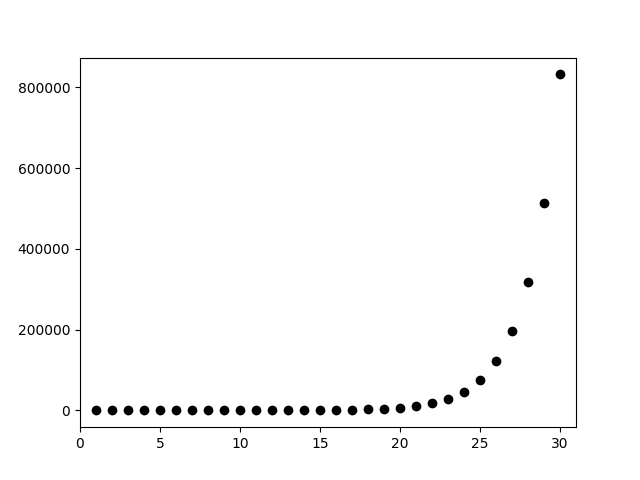
\includegraphics[width = 0.55\textwidth]{./assets/imgs/fibonacci.png}
\caption{Les 30 premières valeurs de la suite de Fibonacci}
\label{fig:fibonacci}
\end{figure}

Dans l'image \ref{fig:fibonacci}, on peut observer la croissance rapide de la suite de Fibonacci. Peu importe la ligne horizontale qu'on tracerait sur ce graphe, la suite va forcément la dépasser !

\section{Suites numériques}

Pour définir une suite, au sens de la Définition \ref{def:suite}, de manière rigoureuse, il y a 3 manières~:

\begin{enumerate}
    \item La suite est définie \emph{par récurrence}~: le $n$-ième élément $x_n$ est défini en fonction d'autres éléments $x_i$ avec des indices $i < n$. C'est le cas de la suite de Fibonacci étudiée précédemment~: $x_n = x_{n-1} + x_{n-2}$ pour $n \geq 3$ avec $x_1 = x_2 = 1$ comme point de départ. Il est important de bien donner les éléments initiaux de la suite, car ils ne peuvent pas être définis en termes d'autres éléments.
    \item La suite est définie explicitement~: le $n$-ième élément $x_n$ est une fonction de $n$. Par exemple, $x_n = n^2 + n - 2$ pour tout $n \geq 1$.
    \item La suite est définie par une propriété non-ambiguë~: par exemple, $x_n$ est le $n$-ième nombre premier.
\end{enumerate}

Les suites peuvent exhiber des propriétés diverses et variées. Il n'y a pas de règle générale permettant de décrire le comportement de toutes les suites en même temps. Voici néanmoins quelques exemples de comportements que l'on peut observer~:

\begin{enumerate}
    \item La suite de Fibonacci est croissante, non-bornée.
    \item La suite $x_n = (-1)^n$ est bornée, mais n'est ni croissante, ni décroissante. La suite alterne entre les valeurs $-1$ et $+1$.
    \item La suite $x_n = (-1)^n \cdot n$ est non-bornée, ni croissante, ni décroissante.
    \item La suite $x_n = \frac{1}{n}$ pour $n \geq 1$ est bornée car $-1 \leq x_n \leq 1$ pour tout $n \geq 1$, et elle est aussi décroissante.
\end{enumerate}

Étudions plus en détail le dernier exemple, $x_n = \frac{1}{n}$. Si on calcule les premiers termes explicitement, on observe le comportement suivant~: 

\begin{figure}[H]
\centering 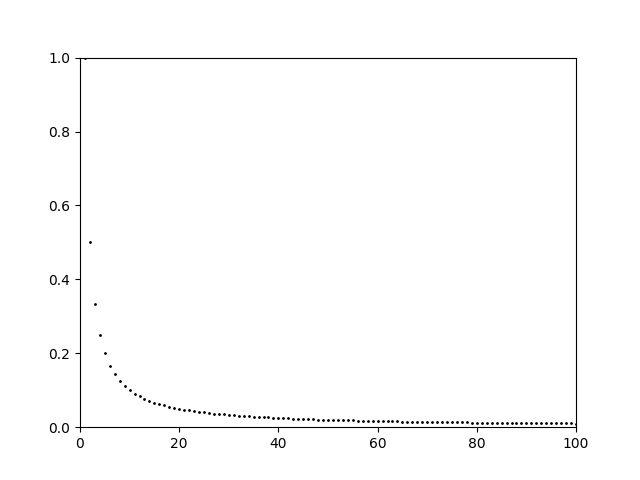
\includegraphics[width = 0.55\textwidth]{./assets/imgs/1_sur_n.png}
\caption{Les 100 premières valeurs de la suite $x_n = \frac{1}{n}$}
\label{fig:1_sur_n}
\end{figure}

On observe que plus $n$ devient grand, plus $\frac{1}{n}$ devient petit et se rapproche de $0$. Cela motive la définition (informelle) suivante~:

\begin{boxdef}[Convergence d'une suite (informelle)]
On dit qu'une suite $(x_n)_{n \geq 1}$ \emph{converge} vers un nombre $l \in \mathbb R$ si, en ignorant suffisamment de termes initiaux $x_1, x_2, ..., x_{n_0}$, \emph{tous} les éléments restants de la suite sont aussi proches de $l$ que l'on veut. On dit que $l$ est la \emph{limite} de la suite $(x_n)$ et on note 
\[
\lim \limits_{n \to \infty} x_n \eqdef l
\]

Si un tel nombre $l \in \mathbb R$ n'existe pas, on dit que la suite \emph{diverge}.
\label{def:convergence}
\end{boxdef}

Intuitivement, comme pour la suite $x_n = \frac{1}{n}$, cela signifie que lorsque $n$ est arbitrairement grand, $x_n$ devient arbitrairement proche de sa limite $l$ ($l = 0$ pour $x_n = \frac{1}{n}$). 

Reprenons à nouveau quelques exemples~:

\begin{enumerate}
    \item La suite de Fibonacci diverge. En effet, la propriété $x_n \geq n-1$ fait qu'on s'éloigne de plus en plus de n'importe quel nombre $l \in \mathbb R$ fixé lorsque $n$ augmente.
    \item La suite $x_n = (-1)^n$ diverge. En effet, on alterne toujours entre $-1$ et $+1$, mais la suite ne se stabilise jamais sur une des deux valeurs.
    \item La suite $x_n = \frac{n+2}{n+1} = 1 + \frac{1}{n+1}$ converge vers $1$.
    \item La suite $x_n = 1$ (suite constante) converge vers $1$.
\end{enumerate}

\section{Propriétés élémentaires des limites}

Avant toute chose, et même si cela peut paraître logique, il faut quand même se poser la question~: est-ce qu'une suite convergente $(x_n)$ peut avoir deux limites distinctes $l_1 \neq l_2$ ?

La réponse est non, c'est-à-dire que

\begin{boxthm}[Unicité de la limite]
La limite d'une suite convergente est \emph{unique}.
\end{boxthm}

En effet, lorsque $n$ devient très grand, la valeur $|x_n-l_1|$ (qui correspond à la distance entre $x_n$ et sa limite $l_1$) peut être rendue aussi proche de $0$ que l'on souhaite. De même, la valeur $|x_n-l_2|$  peut être rendue aussi proche de $0$ que l'on souhaite. On peut alors déduire que
$$|l_1 - l_2| = |(l_1 - x_n) + (x_n - l_2)| \leq |x_n - l_1| + |x_n - l_2| \quad \text{(inégalité triangulaire)}$$ peut être rendue aussi proche de $0$ que l'on souhaite, donc on a nécessairement $l_1 = l_2$.

Il découle également de notre définition informelle que 
\begin{boxthm}[Convergence implique borné]
Toute suite convergente est bornée.
\end{boxthm}

En effet, si $(x_n)$ converge vers $l \in \mathbb R$, alors on peut séparer la suite en des termes initiaux $x_1,x_2,...,x_{n_0}$ et le reste de la suite qui est très proche de $l$, disons au moins à distance $|x_n - l| \leq 1$. Alors
$$|x_n| = |x_n - l + l| \leq |x_n - l| + |l| \leq 1 + |l| \quad \forall n \geq n_0$$ et donc
$$|x_n| \leq \max\{|x_1|, |x_2|, ..., |x_{n_0}|, 1 + |l|\} \quad \forall n \geq 1$$
On a alors trouvé une borne à notre suite.

Logiquement, il découle aussi le résultat suivant

\begin{boxthm}[Non-borné implique divergence]
Toute suite non-bornée est divergente.
\end{boxthm}

En général, une suite bornée n'est pas convergente (e.g. $x_n = (-1)^n$). Cependant, si la suite est monotone (croissante ou décroissante), cela devient vrai.
\begin{boxthm}[Convergence monotone]
Toute suite bornée et monotone est convergente.
\label{thm:conv_monotone}
\end{boxthm}
Par exemple, si la suite $(x_n)$ est croissante et bornée, alors il faut se convaincre qu'on peut trouver une borne supérieure $B \in \mathbb{R}$ telle que $x_n \leq B$ pour tout $n$, et $B$ est choisi le plus petit possible ($B$ devient alors \emph{unique}). Ce $B$ agit alors comme une asymptote horizontale et la suite $(x_n)$, croissante, s'en rapproche petit à petit (cf. Figure \ref{fig:conv_monotone}).

\begin{figure}[H]
\centering 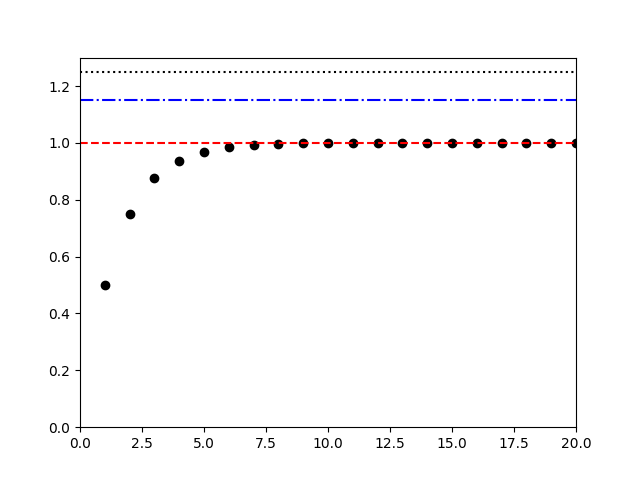
\includegraphics[width = 0.55\textwidth]{./assets/imgs/monotone_convergence.png}
\caption{Illustration de la convergence monotone avec la suite $x_n = 1 - 2^{-n}$. En rouge, on a la borne supérieure la plus petite possible ($B = 1$). En noir et bleu, on a des bornes supérieures plus grandes et donc non-optimales.}
\label{fig:conv_monotone}
\end{figure}

Maintenant, viennent les règles de calculs sur les limites. La première est la linéarité~:

\begin{greybox}
\textbf{Linéarité de la limite.} Soit $(x_n)$ et $(y_n)$ deux suites qui convergent avec limites respectives $\lim \limits_{n \to +\infty}x_n = x$ et $\lim \limits_{n \to +\infty}y_n = y$. Soit $\lambda, \mu \in \mathbb R$ deux nombres réels. Alors la suite $(z_n) = (\lambda \cdot x_n + \mu \cdot y_n)$ converge et sa limite vaut 
$$\lim \limits_{n \to +\infty}(\lambda \cdot x_n + \mu \cdot y_n) = \lambda \cdot \left(\lim \limits_{n \to +\infty}x_n\right) + \mu \cdot \left( \lim \limits_{n \to +\infty}y_n \right) = \lambda \cdot x + \mu \cdot y$$
\end{greybox}

Pour se convaincre de ce résultat, on peut utiliser le raisonnement (informel) suivant~: Lorsque $n$ est très grand, on a $x_n \approx x$, $y_n \approx y$ et donc $\lambda \cdot x_n + \mu \cdot y_n \approx \lambda \cdot x + \mu \cdot y$.

Le même raisonnement permet de se convaincre qu'on a le même comportement avec le produit ou quotient de deux suites convergentes.
\begin{greybox}
\textbf{Produit et quotient de limites.} Soit $(x_n)$ et $(y_n)$ deux suites qui convergent avec limites respectives $\lim \limits_{n \to +\infty}x_n = x$ et $\lim \limits_{n \to +\infty}y_n = y$. Alors~:

\begin{enumerate}
    \item La suite $(z_n) = (x_n \cdot y_n)$ converge et sa limite vaut $$\lim \limits_{n \to +\infty}(x_n \cdot y_n) = \left(\lim \limits_{n \to +\infty} x_n\right) \cdot \left(\lim \limits_{n \to +\infty} y_n\right) = x \cdot y$$
    \item Si $y,y_n \neq 0$ pour tout $n$, la suite $(z_n) = \left(\dfrac{x_n}{y_n}\right)$ converge et sa limite vaut $$\lim \limits_{n \to +\infty}\left( \frac{x_n}{y_n} \right) = \frac{\lim \limits_{n \to +\infty} x_n}{\lim \limits_{n \to +\infty} y_n} = \frac{x}{y}$$
\end{enumerate}
\end{greybox}

\section{Théorème des deux gendarmes}

Le théorème des deux gendarmes permet de déterminer la convergence d'une suite vers une limite $l \in \mathbb R$ grâce à la convergence de deux autres suites vers ce même nombre $l$.

Nous commençons par un cas particulier~:
\begin{boxthm}[Théorème des deux gendarmes : cas particulier]
Soient $(x_n)$ et $(y_n)$ deux suites et $l \in \mathbb R$. Supposons que $l \leq x_n \leq y_n$ pour tout $n$ et que la suite $(y_n)$ converge vers $l$. Alors la suite $(x_n)$ converge aussi vers $l$.
\label{thm:deux_gendarmes_part}
\end{boxthm}

La logique de ce théorème est assez similaire à celle du Théorème \ref{thm:conv_monotone} de convergence monotone. Dans le Théorème  \ref{thm:conv_monotone}, la croissance de la suite $(x_n)$ pousse la suite à converger vers la borne supérieure $B$ la plus petite. Dans notre situation, c'est la suite $(y_n)$ qui remplace la monotonie et va pousser la suite $(x_n)$ vers la borne inférieure $l$.

Du cas particulier, on peut déduire le cas général~:
\begin{boxthm}[Théorème des deux gendarmes]
Soient $(x_n)$, $(y_n)$, $(z_n)$ trois suites. Supposons que $y_n \leq x_n \leq z_n$ pour tout $n$ et que les suites $(y_n)$, $(z_n)$ convergent toutes deux vers une même limite $l \in \mathbb R$. Alors la suite $(x_n)$ converge aussi vers $l$.
\end{boxthm}

Ici, plutôt qu'avoir une borne inférieure fixe comme dans le Théorème \ref{thm:deux_gendarmes_part}, on a une autre suite qui pousse par le bas $(x_n)$ vers la limite $l \in \mathbb R$. Étant donné que $(x_n)$ est aussi poussée par le haut vers $l$, on obtient la convergence.

Comment déduit-on rigoureusement le cas général du cas particulier ? Par hypothèse, on a l'inégalité $0 \leq x_n - y_n \leq z_n - y_n$ pour tout $n$. De plus, $(z_n - y_n)$ converge vers $0$ par linéarité de la limite. Ainsi, le cas particulier implique que $(x_n - y_n)$ converge également vers $0$. En écrivant $x_n = y_n + (x_n - y_n)$, on obtient bien que $x_n$ converge vers $l$ (à nouveau par linéarité de la limite).

Finalement, terminons par un exemple d'application. Prenons la suite $x_n = \frac{\sin(n)}{n}$ pour $n \geq 1$. On se souvient que la fonction sinus donne toujours une valeur comprise entre $-1$ et $1$. Ainsi, on déduit l'inégalité
\[
-\frac{1}{n} \leq \frac{\sin(n)}{n} \leq \frac{1}{n} \quad \forall n \in \mathbb N^*
\]
Les suites $y_n = -\frac{1}{n}$ et $z_n = \frac{1}{n}$ convergent toutes deux vers $0$, donc il en va de même pour la suite $(x_n)$ grâce au Théorème des deux gendarmes.

\section{Théorème d'un gendarme}

Lorsqu'une suite diverge, on distingue un type de divergence particulier : la divergence vers l'infini.

\begin{boxdef}[Divergence d'une suite vers l'infini (informelle)]\label{def:divergence}
On dit qu'une suite $(x_n)_{n \geq 1}$ \emph{diverge vers} $+\infty$ si, en ignorant suffisamment de termes initiaux $x_1, x_2, ..., x_{n_0}$, \emph{tous} les éléments restant de la suite sont positifs et aussi grands que l'on veut. On note 
\[
\lim \limits_{n \to \infty} x_n \eqdef +\infty
\]
Similairement, on dit qu'une suite $(x_n)_{n \geq 1}$ \emph{diverge vers} $-\infty$ si, en ignorant suffisamment de termes initiaux $x_1, x_2, ..., x_{n_0}$, \emph{tous} les éléments restant de la suite sont négatifs et aussi grands (en valeur absolue) que l'on veut. On note 
\[
\lim \limits_{n \to \infty} x_n \eqdef -\infty
\]
\end{boxdef}

Malgré la notation, il faut se rappeler qu'une telle suite ne \textbf{converge pas}. De plus, une suite non-bornée \textbf{ne diverge pas forcément vers} $\pm \infty$ (prendre l'exemple $x_n = (-1)^n \cdot n$).

Un exemple typique de suite qui diverge vers $+\infty$ est donné par $x_n = n$ (ou $x_n = -n$ pour $-\infty$). En effet, si on se donne un $B > 0$ aussi grand que l'on veut, alors à partir de l'indice $n_0 = \lceil B \rceil$, on a $x_n > 0$ et $x_n > B$ pour tous les éléments restants de la suite. En fait, n'importe quelle suite donnée par un polynôme, i.e. $x_n = P(n)$ où $P(x)$ est un polynôme réel, diverge vers $\pm \infty$.

Toutefois, le Théorème \ref{thm:deux_gendarmes_part} est aussi valable, grâce au même raisonnement, pour les suites qui divergent vers l'infini~:

\begin{boxthm}[Théorème d'un gendarme]\label{thm:un_gendarme}
Soient $(x_n)$ et $(y_n)$ deux suites. 

Supposons que $x_n \leq y_n$ pour tout $n$ et que la suite $(y_n)$ diverge vers $-\infty$. Alors la suite $(x_n)$ diverge aussi vers $-\infty$.

Similairement, supposons que $y_n \leq x_n$ pour tout $n$ et que la suite $(y_n)$ diverge vers $+\infty$. Alors la suite $(x_n)$ diverge aussi vers $+\infty$.
\end{boxthm}
De ce théorème et de l'inégalité \ref{eq:fibonacci_lower_bound}, on déduit par exemple que la suite de Fibonacci diverge vers $+\infty$.

\section{Exemples de suites typiques}
Un cas particulier de suites qui revient souvent est la suite de la forme $x_n = \frac{P(n)}{Q(n)}$ où $P(n)$ et $Q(n)$ sont deux polynômes réels et $Q(n) \neq 0$ pour tout $n$. Par exemple, on pourrait avoir les suites
$$x_n = \frac{3n+1}{7n+2}, \quad y_n = \frac{5n^5 - 2n^2 + 9}{4n^3 + 100}, \quad z_n = \frac{8n^2 + n + 1}{12n^7 - 5n^5 + 3}$$
Dans ce genre de cas, la convergence de la suite ne dépend que des termes de plus haut degré des polynômes $P(n)$ et $Q(n)$. En effet, pour $n$ grand, les autres termes sont négligeables en comparaison des termes de plus haut degré (par exemple, $n^2$ est négligeable par rapport à $n^5$). On peut alors (informellement) écrire
$$x_n \approx \frac{3n}{7n} = \frac{3}{7}, \quad y_n \approx \frac{5n^5}{4n^3} = \frac{5n^2}{4}, \quad z_n \approx \frac{8n^2}{12n^7} = \frac{2}{3n^5} \approx 0$$
et cela permet de déterminer $\lim \limits_{n \to +\infty}x_n = \frac{3}{7}$, $\lim \limits_{n \to +\infty}y_n = +\infty$ et $\lim \limits_{n \to +\infty} z_n = 0$.

Un deuxième cas de suites fréquent est la suite géométrique de la forme $x_n = r^n$ pour $r \in \mathbb R$. On peut aussi la définir par récurrence : $x_1 = 1$ et $x_{n} = r x_{n-1}$ pour $n \geq 2$. On distingue plusieurs cas

\begin{enumerate}
    \item Si $r = 1$, il s'agit de la suite constante $x_n = 1$ qui converge vers $1$.
    \item Si $r = -1$, il s'agit de la suite alternée $x_n = (-1)^n$ qui est bornée, mais diverge.
    \item Si $0 \leq r < 1$, la suite est bornée, décroissante et donc elle converge vers un certain $l \in \mathbb R$. L'équation $x_n = r x_{n-1}$ pour tout $n \geq 2$ implique que la limite doit vérifier $l = r \cdot l$, ce qui ne laisse que la possibilité $l = 0$.
    \item Si $-1 < r \leq 0$, la suite se réécrit comme $x_n = (-1)^n |r|^n$ et vérifie
    $$-|r|^n \leq x_n \leq |r|^n$$
    où $0 \leq |r| < 1$ comme dans le cas précédant. La suite converge donc vers $0$ par le théorème des deux gendarmes, mais elle n'est ni croissante, ni décroissante.
    \item Si $r > 1$, la suite diverge vers $+\infty$. Il faut penser à une "croissance exponentielle" vers $+\infty$. Pour s'en convaincre mathématiquement, on peut par exemple prouver l'inégalité de Bernoulli : $r^n \geq 1 + n(r-1)$ lorsque $r > 1$.
    \item Si $r < 1$, la suite est non-bornée et change de signe constamment. Elle diverge. 
\end{enumerate}

\chapter{Séries numériques}
\section{Introduction}
Lorsque l'on additionne plusieurs nombres, on les écrit usuellement avec des symboles "+" entre eux. Cela ne pose pas de problèmes tant que la liste des nombres que l'on ajoute est courte. Cependant, si l'on additionne par exemple les nombres pairs de $2$ à $100$, ou même les nombres de $1$ à $10000$, on devrait en toute logique écrire
\[
S = 2 + 4 + \ldots + 98 + 100
\] sans oublier un seul terme (on a omis la majorité des termes pour éviter de déborder de la feuille). Pour simplifier cette écriture souvent longue, on utilisera une écriture alternative, en utilisant la lettre grecque \textsc{sigma majuscule} $\Sigma$. L'idée est la suivante~:
\begin{enumerate}
    \item On numérote les nombres que l'on veut additionner~: $a_1 = 2, a_2 = 4, \ldots, a_{50} = 100$.
    \item On introduit un \emph{indice de sommation} $k$, qui prend les valeurs $1, 2, \ldots$ jusqu'à $50$
    \item On somme alors les $a_k$ pour toutes les valeurs de $k$.
\end{enumerate}
Ainsi, pour noter la somme des nombres pairs de 2 à 100, on écrit
\[
S = \sum_{k = 1}^{50} a_k = \sum_{k = 1}^{50} 2k
\] où $k$ prend les valeurs de $1$ à $50$, comme indiqué en dessous et au dessus de la somme.

Ce procédé reste valide pour n'importe quelle suite $(a_n)$, en sommant les $n$ premiers termes d'intérêt. Si on prend la suite $(a_n)_{n \geq 1}$ définie par $a_k = 2k$ et qu'on vous demande d'additionner les $50$ premiers termes de la suite, alors on obtient effectivement la somme $S$ comme dans le paragraphe au dessus. De manière générale, tout somme présentée sous la forme $\Sigma$ peut être réécrite comme la somme des $n$ premiers termes d'une suite bien choisie. On appelle ainsi cette somme des $n$ premiers termes d'une suite $(a_n)$ une \emph{somme partielle}.

\section{Série numérique}
\begin{greybox}
Mais pourquoi une somme "partielle" ?
\end{greybox}
Car en effet on somme qu'une partie des termes d'une suite. Or, il existe par construction une infinité de nombres dans une suite, et donc une somme "totale" devrait donc comprendre tous les termes de la suite, c'est-à-dire sommer un nombre infini de termes. Pour ce faire, il nous suffit d'augmenter le nombre de termes de la somme partielle et le faire tendre vers l'infini, en utilisant le concept de \emph{limite}. C'est ainsi que l'on définit une somme infinie, ou \emph{série}, comme la limite de la suite des sommes partielles~:
\begin{boxdef}[Série numérique]
Une série numérique \emph{de terme général $(a_n)$} est un couple de 2 suites~:
\begin{itemize}
    \item La suite $(a_n)_{n \in \mathbb{N}}$ qui est sommée, et
    \item La suite des \emph{sommes partielles} $(S_n)_{n \in \mathbb{N}}$, définie par
    \begin{equation}
    S_n = \sum_{k = 0}^{n} a_k
    \end{equation}
    i.e. $S_n$ est la somme des $n+1$ premiers termes de la suite $(a_n)$.
\end{itemize}
On note alors la \emph{valeur} de la série numérique 
\begin{equation}
\sum_{k=0}^{\infty} a_k \stackrel{\textrm{déf.}}{=} \lim_{n \to \infty} S_n
\end{equation}
quand la limite existe.
\end{boxdef}
Remarquons que l'écriture $\displaystyle\sum_{k = 0}^{\infty} a_k$ possède un sens uniquement si $\displaystyle\lim_{n \to \infty} S_n$ existe, c'est-à-dire si la suite des sommes partielles \emph{converge}.

Cette notion de convergence est très importante car sans elle, il n'y aurait aucun sens à écrire une somme infinie. Pour comprendre plus en détail pourquoi cette notion de convergence est primordiale, prenons l'exemple de la suite $(a_n)_{n \in \mathbb{N}}$ définie par $a_n = (-1)^n$. On a donc
\begin{equation}
S_n = \sum_{k=0}^{n} (-1)^k = \begin{cases}
1 & \textrm{si } n \textrm{ est pair} \\
0 & \textrm{si } n \textrm{ est impair}
\end{cases}
\end{equation}
Or la série numérique de terme général $(a_n)$ a pour valeur
\[
S = \lim_{n \to \infty} S_n \quad \textrm{qui n'existe pas}
\] et donc la somme infinie diverge ; en toute rigueur, l'écriture $\displaystyle\sum_{k = 0}^{\infty} (-1)^k$ n'a pas de valeur définie puisque la limite n'existe pas.

% Avant de passer à la suite, voici quelques définitions qui seront utiles: les séries géométriques ainsi que les séries absolument convergentes.

% \begin{boxdef}[Série géométrique]
% Une \emph{série géométrique} est une série de la forme $\sum_{k=0}^{\infty} ar^k$ avec $a,r \in \mathbb{R}$, où $r$ s'appelle la \textit{raison} de la série. La caractéristique principale qui nous intéresse est sa valeur~:
% \begin{equation}
% \sum_{k=0}^{\infty} a r^k = \left\{
%     \begin{array}{ll}
%         a\frac{1}{1 - r} & \textrm{si } |r| < 1 \\
%         \infty & \textrm{si } r \geq 1 \\
%         \textrm{n'existe pas} & \textrm{sinon}
%     \end{array}
% \right.
% \end{equation}
% \end{boxdef}

% \begin{boxdef}[Série absolument convergente]
% On dit qu'une série de terme général $(a_n)$ est absolument convergente si la série $\displaystyle\sum_{k=0}^{\infty} |a_k|$ converge. Si une série est absolument convergente, alors elle est convergente. 
% \end{boxdef}

\section{Convergence, divergence}
Dans cette section, nous allons introduire plus formellement la notion de convergence des séries numériques, ainsi que les critères de convergence qui nous permettent de trancher plus facilement. Notons que dans la majorité des cas, le calcul explicite de la valeur d'une série est \emph{très complexe}, et ainsi on se contentera dans ce cours de déterminer la convergence ou la divergence de la série.

\begin{boxdef}[Convergence d'une série numérique]
On dit qu'une série numérique $\displaystyle\sum_{k=0}^{\infty} a_k$ converge si et seulement si la suite des sommes partielles $(S_n)$ converge. Si $(S_n)$ est divergente, on dit alors que la série \emph{diverge}.
\end{boxdef}
Cette convergence/divergence d'une série nous apprend des choses en particulier sur le terme général $(a_n)$ de la série. En effet, l'un des théorèmes principaux est que la convergence d'une série implique que la limite du terme général tend vers 0~:
\begin{boxthm}[Condition nécessaire de convergence]\label{thm:condition_necessaire}
Soit $\displaystyle\sum_{k=0}^{\infty} a_k$ la série de terme général $(a_n)_{n \in \mathbb{N}}$. Si la série converge, alors $\displaystyle\lim_{n \to \infty} a_n = 0$.
\end{boxthm}
Ce résultat est notre premier \emph{critère de divergence}~: si $\displaystyle\lim_{n \to \infty} a_n \neq 0$ ou n'existe pas, alors la série diverge. Néanmoins, on ne peut pas l'utiliser comme critère de convergence, c'est-à-dire que $\displaystyle\lim_{n \to \infty} a_n = 0$ n'est pas suffisant pour que la série numérique correspondante converge.

Pour bien comprendre l'intuition de ce théorème, imaginez que votre suite $(a_n)$ tende vers une valeur $a \in \mathbb{R}$ lorsque $n \to \infty$. Cela veut dire lorsque $n$ est grand, $a_n$ est très proche de $a$, de telle sorte que l'on a l'approximation
\begin{equation}
S_n = \sum_{k = 0}^{n} a_k \approx \sum_{k = 0}^{n} a = (n+1)a
\end{equation}
qui a pour limite $\pm\infty$ si $a \neq 0$. Si $\displaystyle\lim_{n \to \infty} a_n$ n'existe pas, alors $S_n$ ne peut pas se stabiliser vers une valeur particulière. On obtient nécessairement alors que $a$ doit être égal à $0$ pour la série puisse converger~; notons cependant que c'est pas une \emph{condition suffisante} pour assurer la convergence, car il existe des exemples de séries avec $\displaystyle\lim_{n \to \infty} a_n = 0$ tel que les sommes partielles divergent (cf. Section \ref{sec:series_exemples}).

\subsection{Critère de comparaison}
Le critère de comparaison est un critère fondamental de convergence des séries, sur lequel de nombreux autres critères sont basés. Il met en oeuvre votre intuition sur la relation d'ordre entre les termes généraux des séries, en utilisant la convergence ou divergence de séries connues.

\begin{boxdef}[Critère de comparaison]
Soient $(a_n), (b_n)$ deux suites numériques, $n_0 \in \mathbb{N}$ tels que~:
\begin{equation}
0 \leq a_n \leq b_n, \quad \forall n \geq n_0
\end{equation}
Alors~:
\begin{itemize}
    \item Si $\displaystyle\sum_{k=0}^{\infty} b_k$ converge, $\displaystyle\sum_{k=0}^{\infty} a_k$ converge.
    \item Si $\displaystyle\sum_{k=0}^{\infty} a_k$ diverge vers $+\infty$, $\displaystyle\sum_{k=0}^{\infty} b_k$ diverge (vers $+\infty$).
\end{itemize}
\end{boxdef}
Notons que la condition que les deux suites soient non-négatives à partir d'un certain rang $n_0$ est primordiale pour que ce résultat soit applicable. En effet, cela implique que la suite des sommes partielles est monotone croissante à partir du rang $n_0$, et puisque la série de terme général $(b_n)$ converge, elle est aussi bornée (par $\displaystyle\sum_{k = 0}^{\infty} b_k$). Ainsi, il nous suffit d'appliquer notre Théorème \ref{thm:conv_monotone} sur la convergence des suites monotones du Chapitre \ref{chap:suite} pour trouver que la série de terme général $(a_n)$ converge de même.

Pour la divergence, notons qu'il se déduit très directement du Théorème d'un gendarme (cf. Théorème \ref{thm:un_gendarme}).

% Imaginez une série dont les sommes partielles sont croissantes mais qui converge éventuellement. Si une autre série a également des sommes partielles croissantes et est \emph{toujours} plus petite que la première série à partir d'un certain rang, alors cette dernière doit forcément converger, sinon elle dépasserait à un moment la première série !

% L'idée derrière la divergence est globalement la même. Considérez ce graphique~:
% \begin{center}
% \begin{tikzpicture}
% \begin{axis}
%     \addplot[blue,only marks] coordinates {
%         (0,0)
%         (1,1)
%         (2,1.9)
%         (3,2.4)
%         (4,3.1)
%         (5,3.6)
%         (6,3.7)
%         (7,3.76)
%         (8,3.764)
%         (9,3.766)
%         (10,3.767) 
%         (11,3.767) 
%         (12,3.767)
%         (13,3.85) 
%         (14,3.85)
%         (15,3.9)
%     };
    
%     \addplot[red,only marks] coordinates {
%         (0,0) 
%         (1,0.6)
%         (2,1.2)
%         (3,1.8) 
%         (4,2.6) 
%         (5,3) 
%         (6,3.2) 
%         (7,3.5) 
%         (8,3.8) 
%         (9,4.2) 
%         (10,4.25) 
%         (11,4.255) 
%         (12,4.255) 
%         (13,4.257) 
%         (14,4.257)
%         (15,4.257)
%     };
% \end{axis}
% \end{tikzpicture}
% \end{center}
% Représentez-vous ce graphique comme 2 séries, bleue et rouge. L'axe $x$ représente le nombre d'éléments parcourus, et l'axe $y$ représente la somme des $x$ premiers termes. On voit qu'à partir de $x = 10$, la série rouge reste supérieur à la bleu~; en assumant qu'on sache que la série rouge converge et que la série bleu ne dépassera jamais après $x = 10$ la série rouge, on peut affirmer que la série bleue \emph{doit} aussi converger ! A contrario, si on sait que la série bleu diverge vers $+\infty$, alors forcément la série rouge va diverger de même, puisqu'elle se trouve au-dessus de la série rouge.

\section{Exemples de séries usuelles}\label{sec:series_exemples}
Dans cette section, on introduit des séries usuelles qui vous seront utiles pour pouvoir appliquer le critère de comparaison.

\begin{boxdef}[Série géométrique]
Une \emph{série géométrique} est une série $S$ de terme général $a_n = a_0 \cdot r^n$, $n \in \mathbb{N}$ et $a_0, r \in \mathbb{R}$~:
\begin{equation}
S = \sum_{n = 0}^{\infty} a_0 \cdot r^n
\end{equation}
$r$ est appelé la \emph{raison} de la série. La série converge si et seulement si $|r| < 1$, auquel cas elle a pour valeur~:
\begin{equation}
\sum_{n = 0}^{\infty} a_0 \cdot r^n = \frac{a_0}{1-r}, \quad |r| < 1
\end{equation}
% Je pense que ce serait un bon exercice de leur faire prouver la formule de la somme partielle, comme l'année dernière
% Si on donne le polycopié à la fin y'a pas de souci à garder le paragraphe, mais ils l'auront probablement avant donc ça donnerait la solution
%
% Notez également que cette équation vient plus généralement du fait que
% \begin{equation}
% \sum_{k=0}^{p} r^n = \frac{1 - r^{p+1}}{1 - r}, \quad |r| < 1    
% \end{equation}
% ce qui fait que si $ p \to \infty $ alors $ r^{p+1} \to 0$ et on retombe sur l'équation du milieu.
\end{boxdef}
Les séries géométriques sont des séries omniprésentes dans tous les domaines mathématiques, qui restent faciles à utiliser.

\begin{boxdef}[Série harmonique]
La \emph{série harmonique} est la série $S$ de terme général $a_n = \frac{1}{n}$, $n \geq 1$~:
\begin{equation}
S = \sum_{n = 1}^{\infty} \frac{1}{n}
\end{equation}
La série harmonique \emph{diverge}, bien que le terme général converge vers $0$.
\end{boxdef}
La série harmonique illustre donc bien pourquoi le Théorème \ref{thm:condition_necessaire} ne marche pas dans le sens inverse, c'est-à-dire pourquoi $\displaystyle\lim_{n \to \infty} a_n = 0$ n'implique pas la convergence de la série numérique associée.

Une généralisation de la série harmonique est faite en changeant la puissance de $n$ dans la fraction, et on obtient alors les \emph{séries de Riemann}~:
\begin{boxdef}[Série de Riemann]
Une \emph{série de Riemann} est une série $\zeta(s)$ de terme général $a_n = \frac{1}{n^s}$, $n \geq 1$ et $s \in \mathbb{R}$~:
\begin{equation}
\zeta(s) = \sum_{n = 1}^{\infty} \frac{1}{n^s}
\end{equation}
La série de Riemann converge si et seulement si $s > 1$. La série harmonique est le cas $s = 1$.
\end{boxdef}
Les séries de Riemann sont primordiales dans l'analyse moderne, et la fonction zêta de Riemann est même l'objet d'un des \href{https://fr.wikipedia.org/wiki/Probl\%C3\%A8mes_du_prix_du_mill\%C3\%A9naire}{7 Problèmes du prix du millénaire} de l'institut Clay. Vous aurez donc l'occasion de les manipuler plus en détail durant le semestre.
\include{content/fonctions-continuité}
\include{content/calcul-différentiel}
\chapter{Les complexes}
% - Rappels sur les ensembles, introduction des ensembles N et R et notation $x \in A$
% - Rappels sur la valeur absolue, distance et inégalité triangulaire

On définit l'ensemble des nombres complexes par : $i^2 = -1$. Cet ensemble est très pratique, car il nous permet de résoudre des équations de type : $x^2 = -3$ qui est non résoluble dans les réels !

Regardons de plus près les concepts principaux de l'analyse complexe :

\section{Fonction complexes}

On dit qu'une fonction 'f' est complexe, si elle est sous la forme suivante : 
$$f(x,y)= u(x,y) + iv(x,y)$$
dans ce cas de figure, on voit clairement que f nécessite deux variables en entrée pour être opérationnelle, à savoir x et y. De la même façon que f va toujours donner en sortie deux valeurs distinctes, une selon i et l'autre sans. On dira que f est une fonction qui par de $R^2$ vers $R^2$ (noté $R^2 \rightarrow R^2$). Ainsi, ce qui rend l'étude des complexes fondamentalement non intuitive, c'est par ce que la fonction requiert quatre dimensions spatiales pour s'exprimer.

les fonctions u et v sont à eux des fonctions réelles qui peuvent, ou non, dépendre de x et y. Mais elles ne sont pas complexes. Elles prennent deux valeurs en entrée, x et y, mais ne donnent qu'une seule valeur de sortie (on note mathématiquement qu'elles sont ($R^2 \rightarrow R$).

En guise d'exemple, on pourrait prendre la fonction suivante : 
$$f(x,y) = x^2 - 3 + i(y - x + 5)$$
Par identification, on voit clairement ici que : 

$$u(x,y) = x^2 - 3 \text{    et   } v(x,y) = y - x + 5$$ 

Si on décide d'évaluer cette fonction en x = 2 et y = 3, on obtient :

$$f(2,3) = 2^2 - 3 +i(3 - 2 + 5) = 4 - 3 + i6 = 1 + 6i$$

Cet exemple illustre bien la nécessité de définir f comme une fonction $R^2 \rightarrow R^2$, elle a pris deux valeurs distinctes en entrée et a recraché deux valeurs distinctes en sorties, qui sont différenciées par le i.

Cette différenciation entre la partie réelle (qui n'est pas attaché à i) et la partie imaginaire (qui est attaché à i) peut-être exploiter afin de rendre notre écriture encore plus intuitive. Les notations suivantes sont toutes équivalentes : 

$$f(2,3) = f(2 + 3i)$$

\subsection{Coordonnées polaires}


Étant donné que nous avons constamment une distinction nette entre l'axe des abscisses et l'axe des ordonnées (x,y) par l'artifice du i. On peut représenter une coordonnée dans l'univers complexe de plusieurs façons, passons les en revues : 

Coordonnées cartésiennes : 

La notation que nous avons introduite jusqu'à présent est dite cartésienne. On la représente de façon suivante, avec $x_p = 2$ et $y_p = 3$. 

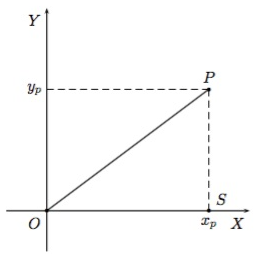
\includegraphics[scale=.5]{assets/imgs/complexe.png}

Coordonnées polaires :

Une autre façon de se représenter un point dans un espace en deux dimensions, c'est de visualiser le mouvement, non pas comme une évolution le long des coordonnées cartésiennes respectives, par exemple le point (2,3) qui va aller vers (4,3) puis vers (4,7). Une première translation selon x a été faite, puis une seconde le long des ordonnées en y jusqu'à aboutir à la position finale.

On peut observer le mouvement sous une autre forme, lors de cette translation, le point s'est nettement éloigné de l'origine du repère, sa distance entre son emplacement original et final a changé ! En polaire, cette distance est dite radiale (du mot rayon), et on notera cette distance $\rho$. Par la même occasion, ce point en question a changé de coordonnée y, passant de 3 à 7, il est donc monté dans le repère. On peut représenter cette montée mathématiquement par la variation d'un angle qui a augmenté en valeur par rapport à l'axe horizontal. On notera cet angle $\theta$.

Nous aboutissons à un nouveau système de coordonnées, tout autant suffisant pour décrire l'emplacement du point que les coordonnées cartésiennes, sous la forme : $(\rho, \theta)$

$$z = x + iy =  \rho(\cos \phi + i\sin \phi) = \rho e^{i\phi}$$

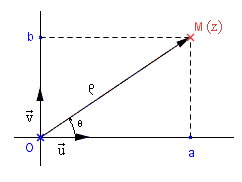
\includegraphics[scale=.5]{assets/imgs/complexe2.png}

\subsection{Rappel notion trigonométrique}

Pour conclure ce bref chapitre, et après avoir rendu compte que les complexes ne sont pas qu'un simple fantasme imaginaire chez les mathématiciens, mais une forme d'analyse à part entière. On vous propose de vous rafraichir la mémoire avec quelques rappels essentiels à fin de pouvoir manipuler l'univers complexe avec aisance, et cela ne peut se faire sans avoir recours à la trigonométrie !

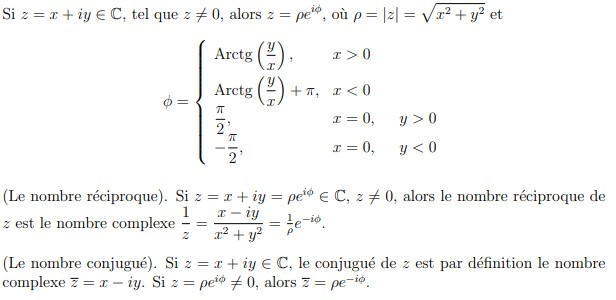
\includegraphics[scale=.7]{assets/imgs/complexe3.jpg}
\newline
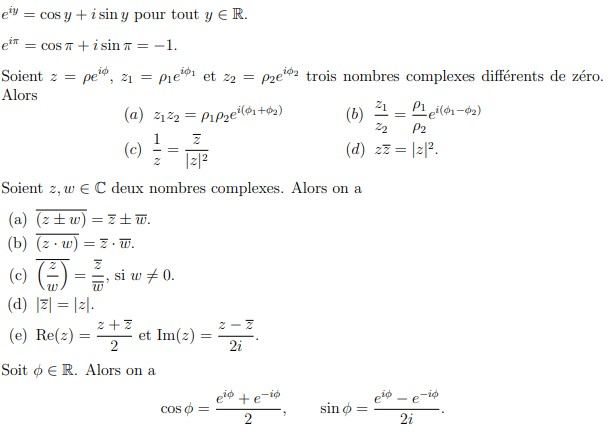
\includegraphics[scale=.7]{assets/imgs/complexe4.jpg}

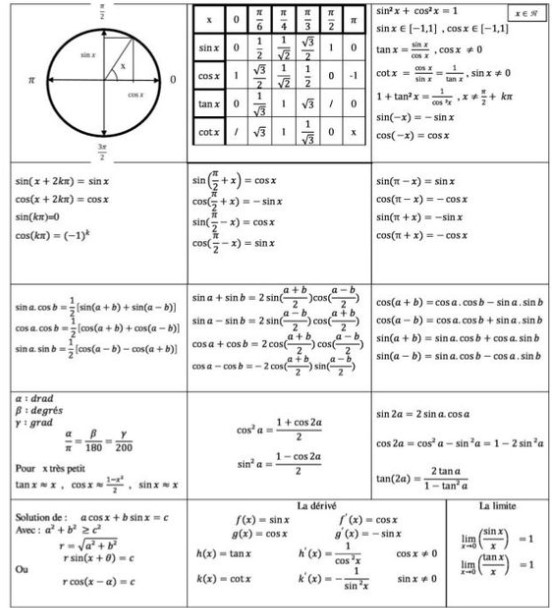
\includegraphics[scale=.8]{assets/imgs/complexe5.jpg}





\end{document}
